\subsection{Algorithmic Optimizations} \label{subsec:algopti}
According to \textcite{shawahna_fpga-based_2019}, 90\% of computation time in \acrshort{cnn} is consumed by the convolution operation. Performing a faster convolution is an approach to reduce the computational complexity of \acrshort{cnn}.
%
%
\subsubsection{GEMM}
%
%
\acrfull{gemm} is a common way to process \acrshort{cnn} on \acrshort{cpu} and \acrshort{gpu} \cite{abdelouahab_accelerating_2018}. We convert the convolution operation as a matrix-vector multiplication. In other words, we transform the input \acrshort{fm} and the kernels into two 2D matrices. It is done in such a way that the multiplication between those two matrices is the same process as a standard convolution. The \acrshort{gemm} operation can be observed in Figure \ref{fig:gemm}. However, this approach is not suggested for \acrshort{fpga}: \textcite{sze_efficient_2017, zhu_efficient_2020} point out that the \acrshort{fm}s must be copied multiple times when flattened to a vector. It leads to a huge memory footprint and either inefficiency in storage or complex memory management access patterns. Furthermore, it does not reduce the number of operations \cite{liang_evaluating_2020}.
%
\begin{figure}
    \centering
    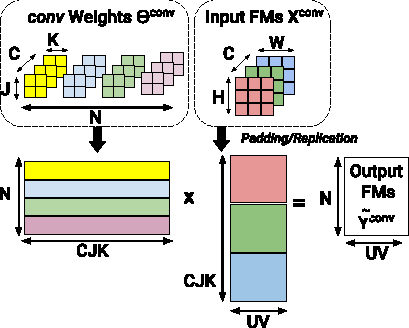
\includegraphics[width=0.5\textwidth]{Images/gemm.pdf}
    \caption{\acrshort{gemm} base processing on convolution layer \cite{abdelouahab_accelerating_2018}}
    \label{fig:gemm}
\end{figure}
%
%
\subsubsection{Fast algorithms for convolution}
%
%
As said above, the \acrshort{gemm} can accelerate the convolution but it does not reduce the number of operations. Therefore, we can explore fast convolution algorithms that aim at reducing its arithmetic complexity. According to \textcite{liang_evaluating_2020}, two faster convolution algorithms appeared to be efficient when reducing the arithmetic complexity of 2D convolution: Winograd minimal filter algorithm and \acrfull{fft}. The fast convolution algorithms produce a tile of output instead of a single pixel. Those fast convolutions can also be described by a common formula, that we can observe on Equation \ref{eq:comform}, where $\odot$ is the element-wise multiplication, $T_O, T_I$ the output and input tile.
%
\begin{equation}
    T_O = \boldsymbol{Inv\_Transf} [ \ \boldsymbol{Transf}(T_I) \ \odot \ \boldsymbol{Transf}(Kernel) \ ]
    \label{eq:comform}
\end{equation}
%
\subsubsection{Winograd-based convolution}
%
The Winograd minimal filter algorithm is first introduced by \cite{winograd_arithmetic_1980}. In Winograd filtering algorithm, data is processed by blocs referred to as \textit{tiles}, as following:
\begin{itemize}
    \item An input \acrshort{fm} tile $g$ of size $(N_{ix} \times N_{iy})$ is pre-processed: $$\boldsymbol{Transform}(T_I) = \boldsymbol{G^{T}} T_I \boldsymbol{G} $$
    \item In the same way, $Kernel$, of size $(K_x \times K_y)$ is also transformed: $$\boldsymbol{Transform}(Kernel) = \boldsymbol{B^{T}} Kernel \boldsymbol{B}$$
    \item The inverse transformation function is then applied to obtain the output tile: $$\boldsymbol{Inverse\_Transform}(E) = \boldsymbol{A^{T}} E \boldsymbol{G}$$ Where $E$ is the result of the element-wise multiplication of the two transformed tiles.
\end{itemize}
The output tile $T_O$ of the Winograd Filtering algorithm, denoted $F(T_{ix} \times T_{iy}, K_x \times K_y)$, is computed using Equation \eqref{eqn:winograd}. The advantage of using the Winograd-based convolution is that the transformation matrix $\boldsymbol{G}$, $\boldsymbol{B}$, $\boldsymbol{A}$ can be computed off-line, using the Winograd Algorithm \cite{winograd_arithmetic_1980}, once $(T_{ix}, T_{iy}, K_x, K_y)$ are fixed. As a result, these transforms become multiplications with constants and can be optimized on \acrshort{fpga} \cite{liang_evaluating_2020}.
%
\begin{equation}
    T_O = \boldsymbol{A^{T}} [ \ \boldsymbol{G^{T}} T_I \boldsymbol{G} \odot \boldsymbol{B^{T}} Kernel \boldsymbol{B} \ ] \boldsymbol{A}
    \label{eqn:winograd}
\end{equation}

According to \textcite{winograd_arithmetic_1980}, the winograd convolution reduces the number of multiplications at the cost of an increase in the numbers of additions. We can observe the gain in Equation \eqref{eq:winograd_gain}. For example, if $T_{ix} = T_{iy} = 2$ and $N_{kx} = N_{ky} = 3$, the complexity reduction $F_{multiplication} = 2.25$ \cite{lavin_fast_2015}.
%
\begin{equation}
    F_{multiplication} = \frac{T_{ix} \times T_{iy} \times N_{kx} \times N_{ky}}{(T_{ix} + N_{kx} - 1) \times (T_{iy} + N_{ky} - 1)}
    \label{eq:winograd_gain}
\end{equation}
%
\subsubsection{FFT-based convolution}
%
The \acrshort{fft}, introduced by \textcite{cooley_algorithm_1965}, is an algorithm to transform the tile into the frequency domain. It can be integrated into the convolution to reduce the number of operations, where:
\begin{itemize}
    \item $\boldsymbol{Transf(*)} = FFT(*)$
    \item $\boldsymbol{Inverse\_Transform(*)} = IFFT(*)$
\end{itemize}
%
Using \acrshort{fft}, the computational complexity can be reduced from $O(N_{ix} \times N_{iy} \times N_{kx} \times N_{ky})$ to $O(N_{i\{x,y\}} log_2(N_{k\{x,y\}}))$ \cite{w_smith_scientist_1997}.
%
\subsubsection{Comparison between the two fast convolutions}
%
Winograd-based convolution seems to be a preferred way to perform fast convolution. This is explained by three reasons: first, \textcite{lavin_fast_2015} demonstrated that Winograd convolution is efficient when the kernel is small ($K_* \leq 3$) and small stride; second, \acrshort{fft}-based convolution is more adequate when the kernel is large \cite{ahmad_towards_2019, chitsaz_acceleration_2020}; third, current \acrshort{cnn} trends prior the utilization of small kernel \cite{liang_evaluating_2020, sandler_mobilenetv2_2019}.

Moreover, FPGA implementations of Winograd algorithm have produced good results. For example, \cite{aydonat_opencl_2017, liang_evaluating_2020} utilized Winograd transform and have reduced their computational complexity by around 50\%. However, the Winograd algorithm also has increased the bandwidth utilization \cite{xiao_exploring_2017}.

Yet, \textcite{zeng_optimizing_nodate, chitsaz_acceleration_2020, liang_evaluating_2020} have made works on optimizing the frequency-domain convolution with small filter by using \acrfull{oad} technique \cite{w_smith_scientist_1997} to lower the number of operations and increase the data parallelism.

Desptite those works, according to \textcite{liang_evaluating_2020, podili_fast_2017}, \acrshort{fft} requires more memory, bandwidth, and logic resources (additions and multiplications) than Winograd. Furthermore, \textcite{zhang_caffeine_2016} pointed that Performing \acrshort{fft} convolution with $1 \times 1$ kernels is inefficient and they have performed it in time-domain only.
